\documentclass{article}

% Language setting
% Replace `english' with e.g. `spanish' to change the document language
\usepackage[english]{babel}
\usepackage{graphicx}
\usepackage{booktabs}
\usepackage{caption}
\usepackage{arydshln}

% Set page size and margins
% Replace `letterpaper' with `a4paper' for UK/EU standard size
\usepackage[letterpaper,top=2cm,bottom=2cm,left=3cm,right=3cm,marginparwidth=1.75cm]{geometry}

% Useful packages
\usepackage{amsmath}
\usepackage{graphicx}
\usepackage[colorlinks=true, allcolors=blue]{hyperref}
\usepackage{tcolorbox}
\title{Bias in Law School Admissions: Analysis and Mitigation Using Machine Learning}
%\author{Federico Marchi, Christina Baytcheva, Anna Di Iulio}
\author{
  Federico Marchi\\
  \texttt{federico.marchi9@studio.unibo.it}
  \and
  Christina Baytcheva\\
  \texttt{christina.baytcheva@studio.unibo.it}
  \and
  Anna Di Iulio\\
  \texttt{anna.diiulio@studio.unibo.it}
}
\begin{document}
\maketitle

\begin{abstract}
The legal profession remains one of the least diverse in the U.S., and the bar exam may play a role in that. Exploiting a Law School Admissions dataset from the Law School Admissions Council (LSAC) \cite{lsacdata}, we aim to explore how racial and ethnic disparities manifest in law school bar passage rates. Using publicly available data, we plan to examine whether schools with higher percentages of students from underrepresented racial and ethnic backgrounds tend to have lower first-time bar exam pass rates, even when controlling for academic and institutional factors. Our goal is to analyze potential sources of bias, test machine learning models for fairness, and explore strategies to reduce algorithmic and systemic inequities.

\end{abstract}

\section{Introduction}

The bar exam plays a critical role in determining who enters the legal profession, yet it may also reflect broader racial and systemic inequalities. This project will use student-level data to explore how racial and ethnic disparities influence bar passage rates. Through exploratory data analysis and the application of machine learning classification models (pass vs. fail), we aim to identify patterns of bias and assess the extent to which these models inherit or amplify existing inequities in the data. Finally, we will test bias mitigation techniques to evaluate whether more balanced and fair predictions can be achieved without significantly compromising model performance.

\section{Background and Motivation}
We recognize the importance of studying the fairness of algorithms in the educational context as it is of high relevance in today's world, and it is necessary to achieve results which are acceptable in order to maintain equality and non-discrimination in this field, and make sure everyone is given a fair chance regardless of their features. 

Previous studies have conducted similar research by training models to assess how bias is learned and to what extent mild bias contained in the dataset can have a heavy influence on the bias after the prediction model(\href{https://www.researchgate.net/publication/387044808_Fair_and_Transparent_Student_Admission_Prediction_Using_Machine_Learning_Models#read}{Fair and Transparent Student Admission Prediction Using Machine Learning Models}). Furthermore, it is interesting to see how the models we are going to develop in this study are going to reflect on a different dataset from a different country, to see if transfer learning is possible(\href{paper-2024-ull-dataset-benchmark.pdf}{Unfair Inequality in Education: A Benchmark for AI-Fairness Research}).



\section{Dataset}
The chosen dataset is available on Kaggle at the following link: 
\href{https://www.kaggle.com/datasets/danofer/law-school-admissions-bar-passage/data}{law school admission dataset}, and it is a snapshot of the  Law School Admissions dataset from the Law School Admissions Council (LSAC). To this day, it is the largest dataset that exists which contains demographic and academic information about aspiring lawyers, and even if it was created in 1998 it is still relevant. 

The contained information, as previously mentioned, is both demographic and academic. In the demographic subset of features we mainly find two:
\begin{enumerate}
    \item gender - which is encoded in a one-hot way in the "male" column
    \item race - which groups individuals in five categories: white, black, asian, hispanic and other
    \item age - this column appeared to have random values inside, ranging from 10 to 70, therefore it was not considered meaningful for analysis. According to statistics, the average age at which people sit the bar exam is around 31 years old, which here only has 11 entries.
    \item birth year - same goes for birth year, which was again dropped.
    \item family income - this divides the candidates into 5 income buckets, where the group 5 represents the richest people, and 1 the poorest. 
\end{enumerate}
In the academic subset instead we find: 
\begin{enumerate}
    \item deciles - represent in which percentage the students are located in terms of academic career during law school. So we need to check for their values and their correlation with gpa
    \item gpa and ugpa -  the undergraduate gpa (identical according to correlation matrix)
    \item zgpa - the standardized final law school GPA
    \item lsat - the lsat score that a student got. Some manipluation was probably performed when the data was entered in the database, as the values of an LSAT exam range from 120 to 180, which is not the case here.
    \item zfygpa - the standardized first-year law GPA
    \item fulltime - indicates how a candidate attended school, as a full time or part time student. 
    \item dropout - flag that indicates if a person has dropped out of school. Contains three values, Y (they did graduate), X (they did not graduate) and O (other)
    \item bar - indicates the outcomes of the first and second attempt at the bar exam. 
    \item tier - represents how exclusive and selective the school the candidate attended is. We have a total of 6 tiers, with 6 being the highest
\end{enumerate}

The dataset also contains multiple extremely ambiguous features which are completely excluded in final analysis, as they seem to hold no real meaning or correlation to the target variable. 

Furthermore, the choice of this specific dataset was made as it contained the ground truth as well, which made it interesting from the machine learning point of view as it enabled us to check the effectiveness of the models before and after bias mitigation. 

\section{Description}

\subsection{EDA}
Exploratory Data Analysis is the initial step in the data analysis process where analysts examine datasets to summarize their main characteristics, often using visual methods. The goal is to understand the structure, detect anomalies, identify patterns, test assumptions, and gain insights that inform further analysis. EDA helps ensure data quality and guides the selection of appropriate modeling techniques.

The findings for this section are extremely important to identify where bias might be located, as it is usually linked to places where the distribution of the features is extremely unbalanced. Through visualization we were able to uncover the following insights. 
\begin{enumerate}
    \item As previously mentioned, only around 1.1k students out of the 22k present in the dataset, receive a Fail score oon the exam. This means that due to the heavy unbalanced nature of the true label, the models are going to struggle to make the correct predictions. This is going to be further explained in subsection 4.3.
    \item In our dataset, we have a balanced number of men and women, and this fairness is extended in the distribution of the ground truth, meaning almost the same percentage of men and women pass or fail the exam. 
    \begin{figure}[h!]
      \centering
      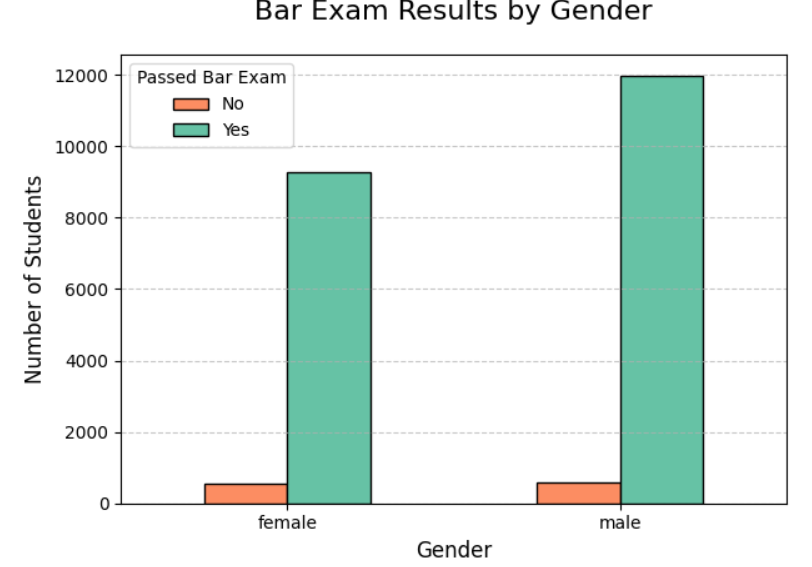
\includegraphics[width=0.5\textwidth]{bar_exam_results_gender.png} 
      \caption{Bar exam results by gender}
      \label{fig:example}
    \end{figure}
    \item It was noticed that the race feature presents heavy imbalance, as the great majority of candidates appear to be white. Black is the second most represented group, but the gap between the two is significant.
    \noindent
    \begin{center}
      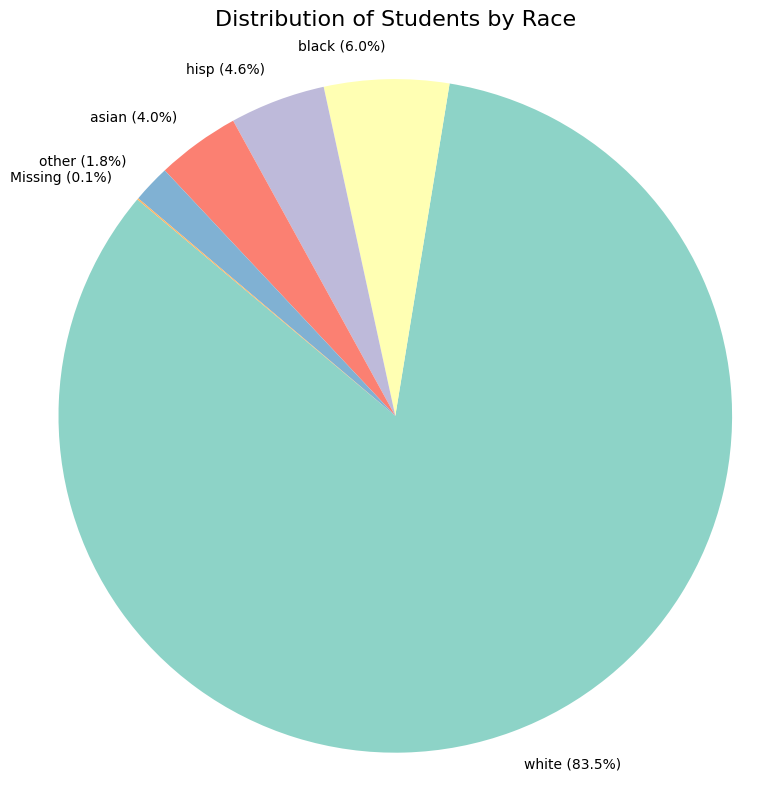
\includegraphics[width=0.5\textwidth]{race_distribution.png}
      \vspace{0.5em}
      \textbf{Figure:} Distribution of Race feature
    \end{center}
    Even more concerning, is the fact that while being the second most represented groups, black students are the ones which seem to be less likely to pass the exam, as evident from the following table:
    \begin{table}[h!]
    \centering
    \caption{Pass Rates by Race}
    \begin{tabular}{lrrr}
    \toprule
    Race & Total Students & Passed & Pass Rate (\%) \\
    \midrule
    White   & 18,713 & 18,084 & 96.638700 \\
    Asian   & 897    & 827    & 92.196210 \\
    Other   & 408    & 366    & 89.705882 \\
    Hispanic & 1,027  & 899    & 87.536514 \\
    Black   & 1,342  & 1,044  & 77.794337 \\
    \bottomrule
    \end{tabular}
    \label{tab:pass_rates_race}
    \end{table}
    \item Any of the variables concerning grades and gpa do not seem to have an unexpected distribution. They were aggregated in a single feature called 'academic career', through a standard scaler, and the results show two normal distributions which have peaks in different places (lower grades = less likely to pass the exam, higher grades = more likely to pass the exam). This is exactly what should be expected from such a variable. 
    \noindent
    \begin{center}
      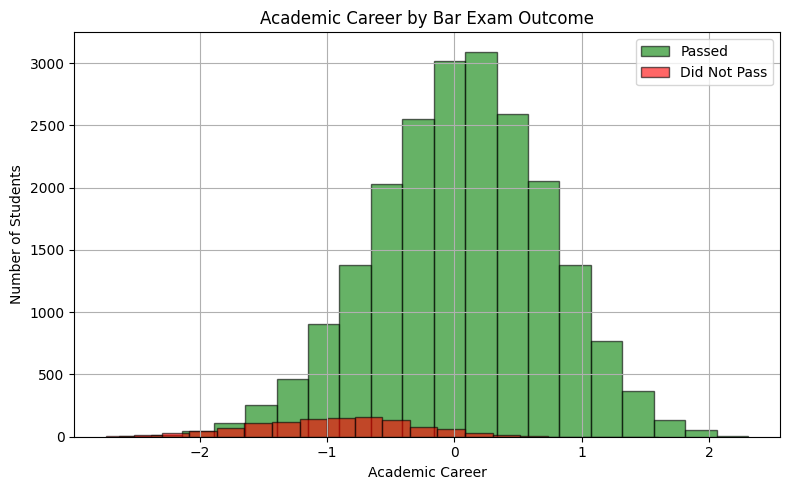
\includegraphics[width=0.5\textwidth]{academic-career.png}
      \vspace{0.5em}
      \textbf{Figure:} Distribution of pass fail outcomes by academic career
    \end{center}
    \item The pass bar variable is divided up into bar1 and bar2 which encodings of the bar column to know wether a student has passed the exam at the first or second try. This shows that:
    \begin{itemize}
        \item 19796 students have passed the bar exam on their first try
        \item 1393 have passed at the second try (19796+1393 = 21189)
        \item 1161 students do not pass the exam at all
    \end{itemize}
    \item The family income distribution is unbalanced in a similar way to race, but in this case it is noticeable how group 5, which is the second to last in terms of number of elements, still has the highest pass rate. 
    \noindent
    \begin{center}
      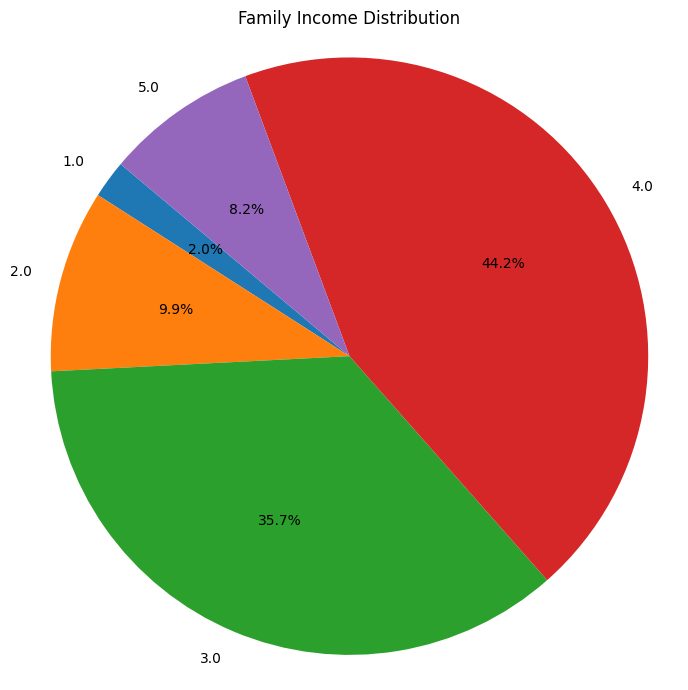
\includegraphics[width=0.5\textwidth]{family income distribution.png}
      \vspace{0.5em}
      \textbf{Figure:} Distribution of family income
    \end{center}
    \begin{table}[h!]
    \centering
    \caption{Pass Rates by Family Income Group}
    \begin{tabular}{lrrr}
    \toprule
    Family Income Level & Total Students & Passed & Pass Rate (\%) \\
    \midrule
    5.0 & 1,813 & 1,745 & 96.249311 \\
    4.0 & 9,748 & 9,374 & 96.163316 \\
    3.0 & 7,880 & 7,436 & 94.365482 \\
    2.0 & 2,179 & 1,989 & 91.280404 \\
    1.0 & 452   & 389   & 86.061947 \\
    \bottomrule
    \end{tabular}
    \label{tab:pass_rates_income}
    \end{table}
    \item In terms of school tier, the exact same phenomenon is observed. As previously stated, tier 6 schools are the most selective, while tier 1 are the least. 
    \noindent
    \begin{center}
      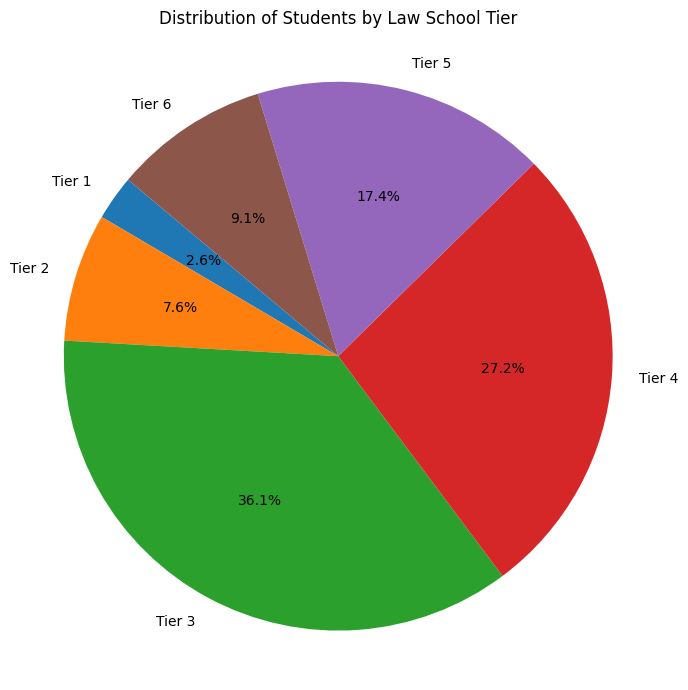
\includegraphics[width=0.5\textwidth]{tier.png}
      \vspace{0.5em}
      \textbf{Figure:} Distribution of school tier
    \end{center}
    \begin{table}[h!]
    \centering
    \caption{Pass Rates by Tier}
    \begin{tabular}{lrrr}
    \toprule
    Tier & Total Students & Passed & Pass Rate (\%) \\
    \midrule
    1.0 & 591   & 460   & 77.834179 \\
    2.0 & 1,690 & 1,550 & 91.715976 \\
    3.0 & 8,073 & 7,640 & 94.636442 \\
    4.0 & 6,069 & 5,827 & 96.012523 \\
    5.0 & 3,882 & 3,703 & 95.388975 \\
    6.0 & 2,045 & 2,009 & 98.239609 \\
    \bottomrule
    \end{tabular}
    \label{tab:pass_rates_tier}
    \end{table}
\end{enumerate}
This EDA has therefore pointed out which are the features which are possible vessels of bias, and need to be investigated through the proper techniques illustrated in the following section. 
These features are:
\begin{itemize}
    \item race
    \item family income
    \item school tier
\end{itemize}
\noindent
\subsection{First Bias Detection}
To detect potential biases in law school admissions, we analyzed the Law School Admission dataset across key demographic variables: gender, race, family income, and undergraduate institution tier. We adopted a hybrid evaluation approach, combining traditional group fairness indicators and a distributional analysis using Wasserstein distance. Specifically, we relied on AIF360 metrics like Disparate Impact to assess disparities across demographic categories. However, this method typically focus on discrete classifications and may fail to capture deeper structural imbalances. To address this, we integrated Wasserstein distance to examine how the distribution of outcomes shifts across groups—highlighting subtler, systemic biases that group-based metrics might miss. By uniting these two perspectives, we aimed to achieve a more robust and layered understanding of fairness in the admissions data. As protected attributes we used male for gender, white for race, group 5 (high income) for family income and group 6 (most selective school) for tier; these were compared to all other groups, so that we can see if there is any bias compared to the privileged group. Our findings across the different methods and categories can be summarized in this table:

\begin{center}
\captionof{table}{Initial Bias Detection}
\begin{tabular}{llrrr}
\toprule
Attribute & Group & Disparate Impact & Wasserstein Dist. \\
\midrule
\textbf{Gender}
& female & 0.98 & 0.0095 \\
\midrule
\textbf{Race}
& black & 0.81 & 0.1896 \\
& hisp & 0.91 & 0.0915 \\
& asian & 0.95 & 0.0444 \\
& other & 0.93 &  0.0707 \\
\midrule
\textbf{Family Income}
& 1.0 & 0.89 & 0.1019 \\
& 2.0 & 0.95 & 0.0497 \\
& 3.0 & 0.98 & 0.0188 \\
& 4.0 & 1.00 & 0.0009 \\
\midrule
\textbf{Tier}
& 1 & 0.80 & 0.1974 \\
& 2 & 0.93 & 0.0664 \\
& 3 & 0.96 & 0.0360 \\
& 4 & 0.98 & 0.0226 \\
& 5 & 0.97 & 0.0282 \\
\bottomrule
\end{tabular}
\label{tab:fairness_initial_detection}
\end{center}

We can see that there is no to minimal bias detected for gender and potential bias towards black people when it comes to race. Also, people coming from the lowest family income groups have worse chances compared to the once from the higher; same goes for the tier, students coming from the low tier schools indicate worse success rates compared to their high tier peers.
\subsection{Models and predictions}
For the binary prediction task of determining whether someone passed the bar exam, we selected a linear model, Logistic Regression, and two tree-based models: Random Forest (a bagging method) and XGBoost (a boosting method). Moreover we decided to test a Multi Layer Perceptron since we had available around 20k rows, enough to train a MLP. Let us analyze each of them.
\subsubsection{Logistic Regression}
\paragraph{Baseline and Balanced Models}\mbox{}\\
A baseline model has been trained first, but we immediately noticed the first issue. Since the dataset is extremely unbalanced towards the exam passed, this bring the baseline model to predict in most of the cases that the exam was passed. This means high accuracy, but very low precision and recall values for class 0. Balancing the loss function based on the rate of the two classes, we managed to achieve a better results in the predictions. Follow the two confusion matrices:
\begin{table}[h!]
\centering
\caption{Confusion Matrix for Baseline LR}
\label{tab:confusion_matrix}
\begin{tabular}{r|cc}
\toprule
\textbf{Actual / Predicted} & \textbf{Positive} & \textbf{Negative} \\
\midrule
\textbf{Positive} & 25 & 202 \\
\textbf{Negative} & 18 & 4170\\
\bottomrule
\end{tabular}
\end{table}

\begin{table}[h!]
\centering
\caption{Confusion Matrix for Balanced LR}
\label{tab:confusion_matrix}
\begin{tabular}{r|cc}
\toprule
\textbf{Actual / Predicted} & \textbf{Positive} & \textbf{Negative} \\
\midrule
\textbf{Positive} & 189 & 38 \\
\textbf{Negative} & 913 & 3275 \\
\bottomrule
\end{tabular}
\end{table}
As shown, the current model predicts a significantly higher number of passed exams compared to the baseline. However, this improvement comes at the cost of a substantial increase in false negatives, students who did not pass but were predicted to have passed. \newline
\paragraph{Grid Search based on F-Beta score}\mbox{}\\
In our context, it is crucial that the model identifies a reasonable number of students who did not pass the exam (i.e., the minority class). If the model fails to predict these cases, or predicts too few of them, it undermines the purpose of our study, which is to examine how models embed bias from data. At the same time, we cannot entirely disregard precision, as misclassifying students who actually passed as having failed may carry practical consequences and could introduce new biases.\newline
To address this trade-off, we use the F-beta score, a metric that balances recall and precision, with greater emphasis on recall. Specifically, we adopt the \textbf{F-beta score}, which let us the flexibility in deciding how much importance give to recall and how much to precision. We decided to give twice as much weight to recall compared to precision. This allows us to prioritize identifying as many students who failed as possible, while still maintaining attention to overall prediction accuracy.

\begin{tcolorbox}[colback=gray!5, colframe=gray!80!black, title=F-2 Score]
The F\textsubscript{$\beta$} score is a weighted harmonic mean of precision and recall, defined as:
\[
F_{\beta} = (1 + \beta^2) \cdot \frac{\text{Precision} \cdot \text{Recall}}{(\beta^2 \cdot \text{Precision}) + \text{Recall}}
\]
When $\beta = 2$, recall is weighted twice as heavily as precision:
\[
F_2 = 5 \cdot \frac{\text{Precision} \cdot \text{Recall}}{4 \cdot \text{Precision} + \text{Recall}}
\]
\end{tcolorbox}
\mbox{}\newline
We then performed a \textbf{Grid Search} over different class weights and regularization parameters, achieving a well-balanced compromise. The best model we achieved is the one which uses moderate regularization (\texttt{C=1}) and increases the weight of the minority class (class 0) by a factor of 5 to improve its recall.\\We also tried tuning the threshold based on the same metric, but the default one results to be the best one. Below is the confusion matrix of the model we considered the best, based on its F-beta score. 
\begin{table}[h!]
\centering
\caption{Confusion Matrix for Best LR}
\label{tab:confusion_matrix}
\begin{tabular}{r|cc}
\toprule
\textbf{Actual / Predicted} & \textbf{Positive} & \textbf{Negative} \\
\midrule
\textbf{Positive} & 155 & 72 \\
\textbf{Negative} & 550 & 3638 \\
\bottomrule
\end{tabular}
\end{table}
\paragraph{Overfitting Evaluation}\mbox{} \newline
As shown in the table, the model generalizes well, with no signs of overfitting.
\begin{table}[h!]
\centering
\begin{tabular}{lcccc}
\toprule
\textbf{Class} & \textbf{Precision} & \textbf{Recall} & \textbf{F1-Score} & \textbf{Support} \\
\midrule
0 (test) & 0.22 & 0.68 & 0.33 & 227 \\
1 (test) & 0.98 & 0.87 & 0.92 & 4188 \\[1ex]
\hdashline 
\noalign{\vskip 1ex}  
0 (training) & 0.22 & 0.65 & 0.33 & 912 \\
1 (training) & 0.98 & 0.87 & 0.92 & 16745 \\
\midrule
\end{tabular}
\caption{Performances over test and training set.}
\label{tab:logreg_report}
\end{table}

\subsubsection{Random Forest}
The first tree-based algorithm we decided to test is Random Forest. While not as simplistic as a standard decision tree, it is still not the most powerful among tree-based models. 
\paragraph{Grid Search based on F-Beta score}\mbox{}\newline
We performed a grid search over the parameter \texttt{max\_depth} to find the maximum tree depth that allows the model to generalize well. Another parameter we tuned is \texttt{min\_samples\_split}, which specifies the minimum number of samples required to consider splitting a node. Additionally, since we noticed overfitting, we set \texttt{min\_samples\_leaf = 2}, in this way we will force the decision trees within the Random Forest to make splits only when at least two training samples fall into a leaf node, reducing the model’s ability to memorize individual cases.\\ \\
The \textbf{Best Model} we managed to achieve is the one with:
\begin{itemize}
    \item \texttt{max\_depth = 8}
    \item \texttt{min\_samples\_split = 10}
\end{itemize}
Follows the relative Confusion Matrix on the test set:
\begin{table}[h!]
\centering
\caption{Confusion Matrix for Best RF}
\label{tab:confusion_matrix}
\begin{tabular}{r|cc}
\toprule
\textbf{Actual / Predicted} & \textbf{Positive} & \textbf{Negative} \\
\midrule
\textbf{Positive} & 172 & 55 \\
\textbf{Negative} & 719 & 3469 \\
\bottomrule
\end{tabular}
\end{table}
\paragraph{Overfitting Evaluation}\mbox{} \newline
As shown in the table, the model generalizes well, with limited signs of overfitting on class 0:
\begin{table}[h!]
\centering
\begin{tabular}{lcccc}
\toprule
\textbf{Class} & \textbf{Precision} & \textbf{Recall} & \textbf{F1-Score} & \textbf{Support} \\
\midrule
0 (test) & 0.19 & 0.76 & 0.31 & 227 \\
1 (test) & 0.98 & 0.83 & 0.90 & 4188 \\[1ex]
\hdashline 
\noalign{\vskip 1ex}  
0 (training) & 0.22 & 0.84 & 0.35 & 912 \\
1 (training) & 0.99 & 0.84 & 0.91 & 16745 \\
\midrule
\end{tabular}
\end{table}
\subsubsection{XGBoost}
The second tree-based algorithm we tested is XGBoost. While more complex than Random Forest, it is considered one of the most powerful and effective ensemble methods for structured data.
\paragraph{Grid Search based on F-Beta score}\mbox{}\newline
We performed a grid search over the following parameters:
\begin{itemize}
    \item \texttt{n\_estimators} (best value \texttt{= 200}),
    \item \texttt{max\_depth} (best value \texttt{= 7}),
    \item \texttt{learning rate} (best value \texttt{= 0.1}),
    \item \texttt{gamma}, which is the minimum loss reduction in order to split  (best value \texttt{= 0}).
\end{itemize}
Follows the relative Confusion Matrix on the test set:
\begin{table}[h!]
\centering
\caption{Confusion Matrix for Best XGBoost}
\label{tab:confusion_matrix}
\begin{tabular}{r|cc}
\toprule
\textbf{Actual / Predicted} & \textbf{Positive} & \textbf{Negative} \\
\midrule
\textbf{Positive} & 186 & 41 \\
\textbf{Negative} & 868 & 3320 \\
\bottomrule
\end{tabular}
\end{table}
\paragraph{Overfitting Evaluation}\mbox{} \newline
At first we noticed some overfitting over the training set, in order to reduce it we applied both: 
\begin{itemize}
    \item \textbf{L1 regularization}: helps in pushing some leaf weights to zero and encourage sparse trees;
    \item \textbf{L2 regularization}: penalizes large leaf weights, help in avoiding overfitting by reducing the influence of individual trees.
\end{itemize}
Doing so we managed to remove overfitting, the new confusion matrix is:
\begin{table}[h!]
\centering
\caption{Confusion Matrix for Best XGBoost without Overfitting}
\label{tab:confusion_matrix}
\begin{tabular}{r|cc}
\toprule
\textbf{Actual / Predicted} & \textbf{Positive} & \textbf{Negative} \\
\midrule
\textbf{Positive} & 191 & 36 \\
\textbf{Negative} & 927 & 3261 \\
\bottomrule
\end{tabular}
\end{table}
As shown in the table, the model generalizes well, with limited signs of overfitting on class 0:
\begin{table}[h!]
\centering
\begin{tabular}{lcccc}
\toprule
\textbf{Class} & \textbf{Precision} & \textbf{Recall} & \textbf{F1-Score} & \textbf{Support} \\
\midrule
0 (test) & 0.17 & 0.84 & 0.28 & 227 \\
1 (test) & 0.99 & 0.78 & 0.87 & 4188 \\[1ex]
\hdashline 
\noalign{\vskip 1ex}  
0 (training) & 0.18 & 0.89 & 0.30 & 912 \\
1 (training) & 0.99 & 0.78 & 0.88 & 16745 \\
\midrule
\end{tabular}
\end{table}
\subsubsection{MLP}
The final model we tested is a Multi-Layer Perceptron (MLP). Unlike previous methods, this neural network can capture complex non-linear patterns through its multiple layers and activation functions.
\paragraph{MLP architecture}\mbox{}\newline
After scaling numeric features, we have define a MLP with a the following architecture: it consists of an input layer followed by three hidden layers with decreasing sizes (128, 64, and 32 neurons), each using the ReLU activation function. Batch normalization is applied after the first two hidden layers to stabilize and speed up training, and Dropout with a rate of 0.3 is used to reduce overfitting. The final output layer has a single neuron with a sigmoid activation function to classify. \\
It has been used a specific \textbf{Loss Function} in order to address class imbalance by down-weighting well-classified examples and focusing learning on hard, misclassified ones. It has two components:
\begin{itemize}
    \item \textbf{$\gamma$ (gamma)}: controls the strength of down-weighting easy examples. A higher gamma makes the model focus more on hard examples.
    \item \textbf{$\alpha$ (alpha)}: balances the importance of positive vs. negative classes.
\end{itemize}
We then tuned the threshold for prediction based on the define F-beta score. We found that a threshold at \texttt{0.58} gives a better score. 
Follows the relative Confusion Matrix on the test set:
\begin{table}[h!]
\centering
\caption{Confusion Matrix for Best MLP}
\label{tab:confusion_matrix}
\begin{tabular}{r|cc}
\toprule
\textbf{Actual / Predicted} & \textbf{Positive} & \textbf{Negative} \\
\midrule
\textbf{Positive} & 173 & 54 \\
\textbf{Negative} & 721 & 3467 \\
\bottomrule
\end{tabular}
\end{table}
\paragraph{Overfitting Evaluation}\mbox{} \newline
As shown in the table, the model generalizes well, with almost no overfitting:
\begin{table}[h!]
\centering
\begin{tabular}{lcccc}
\toprule
\textbf{Class} & \textbf{Precision} & \textbf{Recall} & \textbf{F1-Score} & \textbf{Support} \\
\midrule
0 (test) & 0.19 & 0.76 & 0.31 & 227 \\
1 (test) & 0.98 & 0.83 & 0.90 & 4188 \\[1ex]
\hdashline 
\noalign{\vskip 1ex}  
0 (training) & 0.20 & 0.77 & 0.32 & 912 \\
1 (training) & 0.99 & 0.83 & 0.90 & 16745 \\
\midrule
\end{tabular}
\caption{Performances over test and training set.}
\label{tab:logreg_report}
\end{table}
\subsubsection{Comparing all models}
\begin{figure}[]
  \centering
  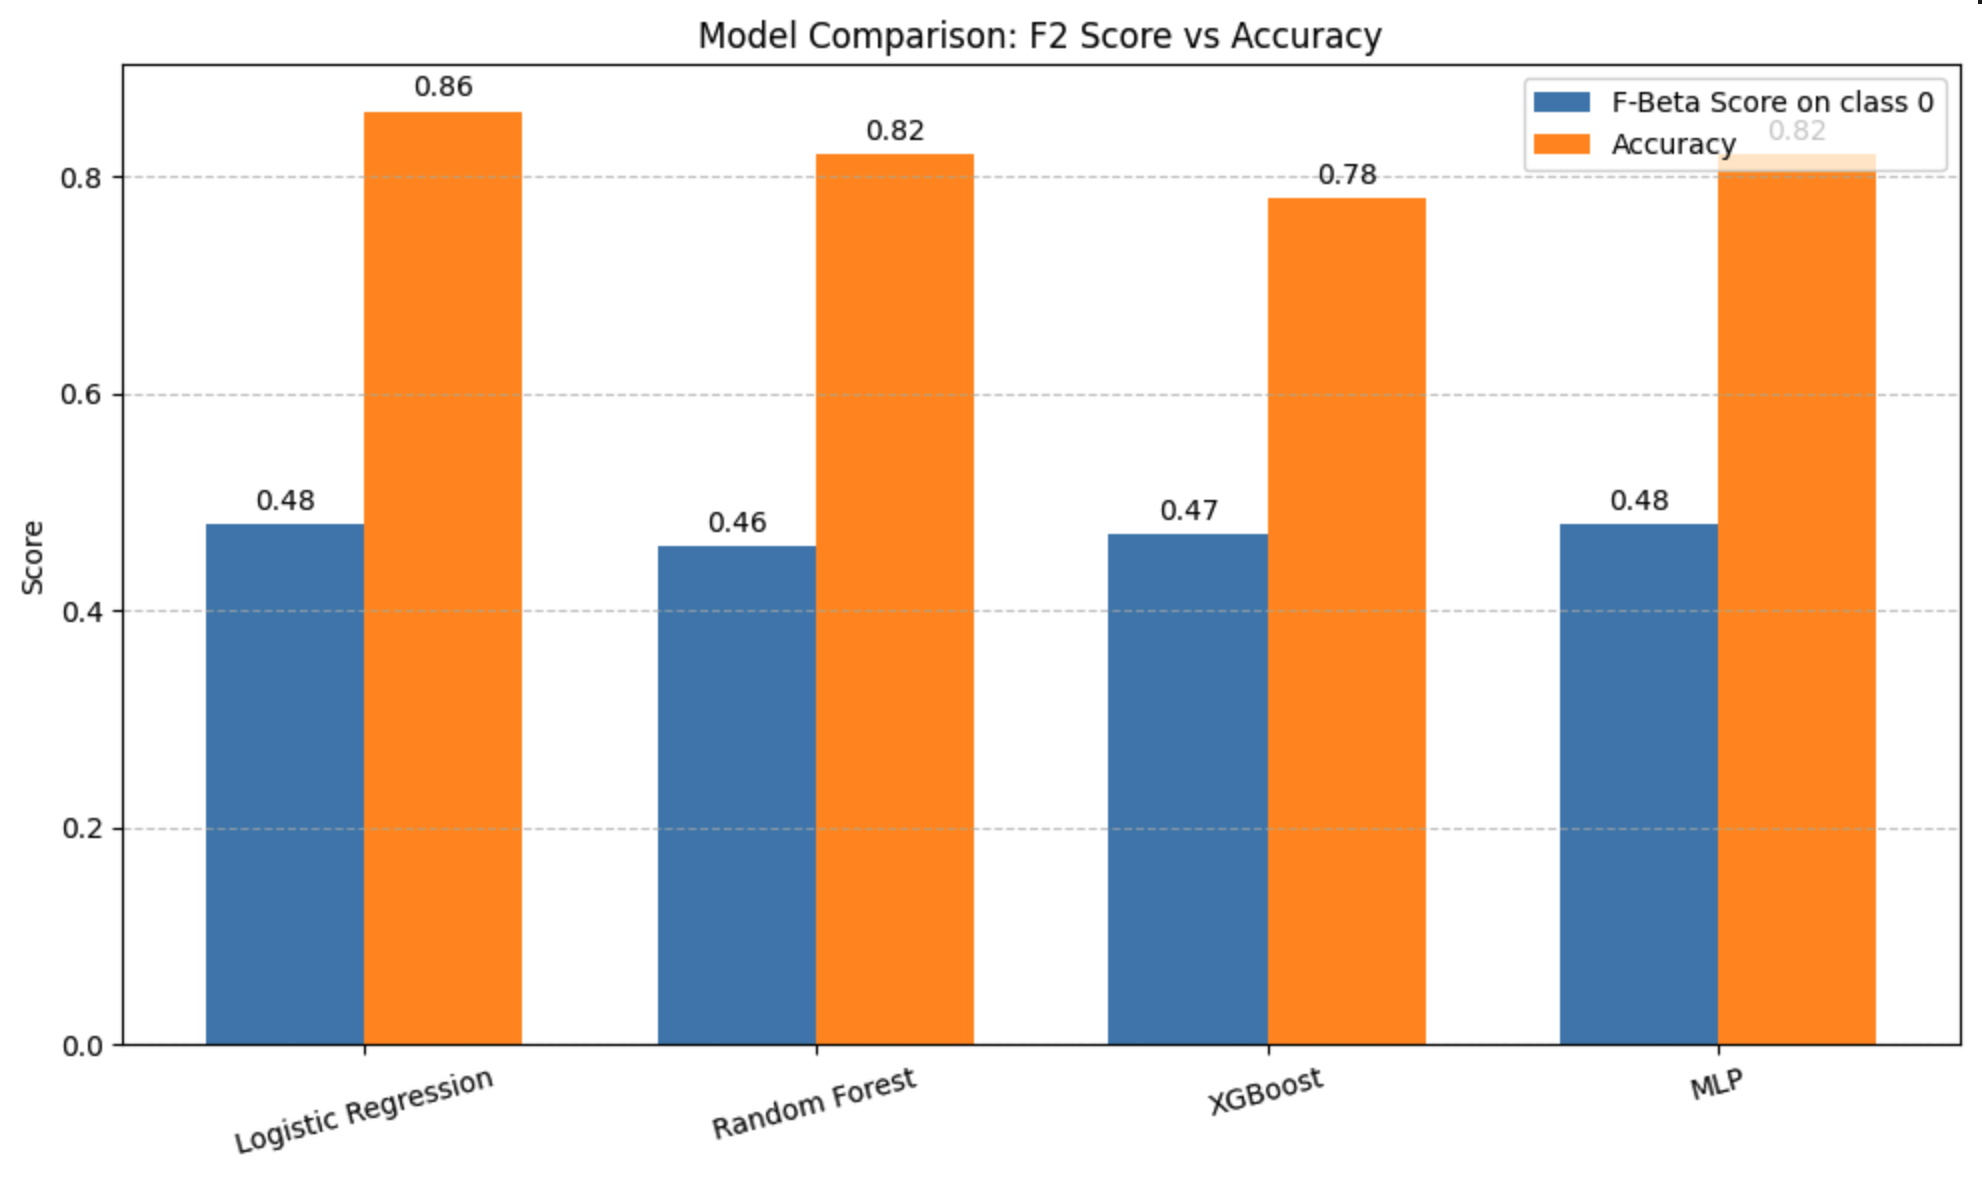
\includegraphics[width=0.8\textwidth]{model_comparison.png}
  \caption{Accuracy and F-beta score for each best model.}
  \label{fig:model_comparison}
\end{figure}
Logistic Regression and MLP have the highest F2 scores (0.48), indicating strong recall on class 0. Logistic Regression also has the best accuracy (0.86), making it the most balanced performer. XGBoost lags in accuracy (0.78), while Random Forest performs slightly lower overall.
\newpage
\subsection{Bias detection after prediction}
After the predictions are performed, it is necessary to check if the new predicted label conveys the same type of bias that is observable in the ground truth variable. When the same analysis is conducted, what is observable is a worsening of the situation in all three features where bias was present. 

As a reminder to interpret the following results:
\begin{itemize}
    \item \textit{Disparate impact}: bias is present if the value is far from 1. In general we apply the 80\% rule, meaning that bias in unacceptable if the disparate impact is below 80\%
    \item \textit{Statistical Parity Difference}: bias is present if the value is far from 0
    \item \textit{Wasserstein Distance}: bias is present if the value is too far from 0
\end{itemize}

The following three tables contain the results of the bias detection method on the predicted label according to the three best models found in the previous step. 

\begin{center}
\captionof{table}{Fairness Metrics by Model and Race compared to White}
\begin{tabular}{llrr} 
\toprule
\textbf{Model} & \textbf{Race} & \textbf{Disparate Impact} & \textbf{Statistical Parity Difference} \\
\midrule
\textbf{Best Logistic Regression} & black & 0.366 & -0.574 \\
 & hisp & 0.611 & -0.352 \\
 & asian & 0.836 & -0.149 \\
 & other & 0.716 & -0.257 \\
\midrule
\textbf{Random Forest} & black & 0.309 & -0.597 \\
 & hisp & 0.609 & -0.338 \\
 & asian & 0.794 & -0.178 \\
 & other & 0.727 & -0.236 \\
\midrule
\textbf{XGBoost R} & black & 0.228 & -0.630 \\
 & hisp & 0.534 & -0.380 \\
 & asian & 0.766 & -0.191 \\
 & other & 0.689 & -0.254 \\
\bottomrule
\end{tabular}
\end{center}

\vspace{1em}

\begin{center}
\captionof{table}{Fairness Metrics by Model and Family Income Group compared to 5}
\begin{tabular}{llrr}
\toprule
\textbf{Model} & \textbf{Income Group} & \textbf{Disparate Impact} & \textbf{Statistical Parity Difference} \\
\midrule
\textbf{Logistic Regression Best}
& 1 & 0.694 & -0.270 \\
& 2 & 0.852 & -0.130 \\
& 3 & 0.932 & -0.060 \\
& 4 & 1.005 & 0.004 \\
\midrule
\textbf{Random Forest}
& 1 & 0.708 & -0.247 \\
& 2 & 0.836 & -0.139 \\
& 3 & 0.916 & -0.072 \\
& 4 & 1.001 & 0.000 \\
\midrule
\textbf{XGBoost R}
& 1 & 0.614 & -0.314 \\
& 2 & 0.778 & -0.180 \\
& 3 & 0.883 & -0.096 \\
& 4 & 0.980 & -0.016 \\
\bottomrule
\end{tabular}
\end{center}

\vspace{1em}

\begin{center}
\captionof{table}{Fairness Metrics by Model and Tier compared to 6}
\begin{tabular}{llrr}
\toprule
\textbf{Model} & \textbf{Income Group} & \textbf{Disparate Impact} & \textbf{Statistical Parity Difference} \
\midrule
\textbf{Logistic Regression Best}
& 1 & 0.568 & -0.415 \
& 2 & 0.747 & -0.242 \
& 3 & 0.846 & -0.147 \
& 4 & 0.916 & -0.081 \
& 5 & 0.938 & -0.060 \
\midrule
\textbf{Random Forest}
& 1 & 0.537 & -0.427 \
& 2 & 0.767 & -0.215 \
& 3 & 0.849 & -0.139 \
& 4 & 0.892 & -0.099 \
& 5 & 0.908 & -0.085 \
\midrule
\textbf{XGBoost R}
& 1 & 0.310 & -0.608 \
& 2 & 0.629 & -0.327 \
& 3 & 0.837 & -0.143 \
& 4 & 0.902 & -0.086 \
& 5 & 0.891 & -0.096 \
\bottomrule
\end{tabular}
\end{center}

\vspace{1em}

These results show that the situation has been worsened significantly by model predictions. This is not unexpected, as recent studies have shown time and time again that models trained on even slightly biased data tend to not only reproduce this bias, but amplify it greatly—as shown in the previous tables. \href{https://arxiv.org/pdf/2201.11706}{source}.
We also observed that bias amplification varies a lot by model. Linear models such as basic logistic regression (the race feature disparate impact is showed below as an example) tend to not learn bias as much as more complex models like XGBoost, but their predictions are unsatisfactory. 

\noindent
\begin{center}
  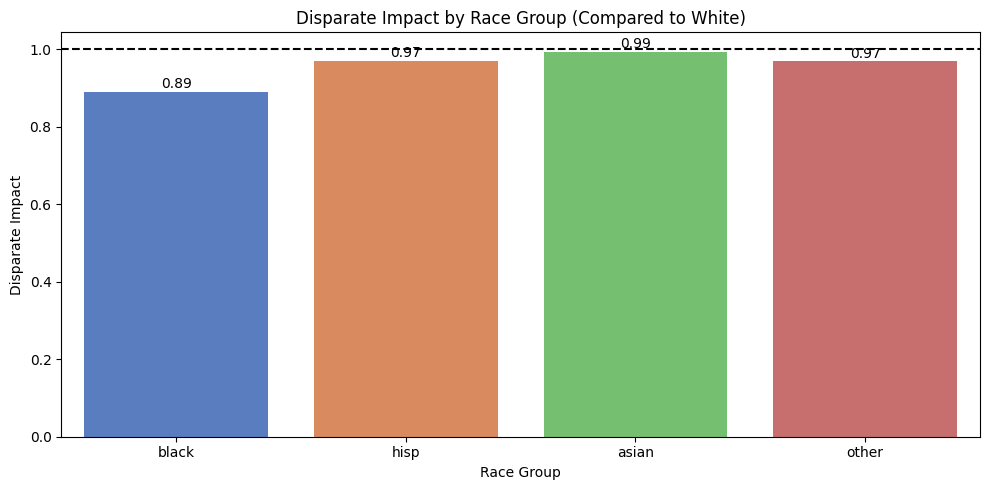
\includegraphics[width=0.5\textwidth]{racelogisticregression.png}
  \vspace{0.5em}
  \textbf{Figure:} Disparate Impact Race Feature Logistic Regression
\end{center}

Therefore, in our specific case we have to tackle two main difficulties: 
\begin{itemize}
    \item the unbalanced nature of the target variable, meaning that most candidates pass the exam. This adds a great deal of difficulty with predictions, as models tend to overfit the majority class and overlook minority cases.
    \item the heavy presence of bias, which needs to be mitigated to ensure fairness and compliance with ethical and legal standards.
\end{itemize}
Both challenges must be addressed simultaneously, as correcting one without considering the other can lead to suboptimal or even harmful outcomes. Developing models that are both accurate and fair requires thoughtful preprocessing, careful model selection, and robust post hoc auditing to detect and correct unfair patterns in predictions.


\subsection{Bias mitigation techniques}
\subsubsection{Preprocessing}
Preprocessing techniques aim to tackle bias at the root, meaning that they operate on the data itself in order to smooth it out as much as possible and, after training the model, the bias should be reduced or overall disappeared. 

The method used is not textbook, but was necessary in order to reduce the bias in a way which made sense, as it was specifically hard to tackle in the preprocessing case. The textbook approaches didn't seem to work at all. The Disparate Impact Remover library from AIF360 is at the moment not working because of technical problems on their side, so we decided to implement a similar approach by hand. 

Disparate Impact is a metric which has a threshold of 1, and we generally enforce the 80\% rule, meaning that if the values drop below 80\% the feature is considered unacceptably biased. DIR is a preprocessing fairness technique which transforms the feature distributions so that protected group membership can no longer be easily inferred. So it alters the ability of the features to be proxies for group identities. More easily, we are hiding where a specific individual belongs to. Another added challenge in this instance was tackling three different features at the same time. It was also proven that using the disparate impact remover on one feature at a time produced worse overall results (80\% rule was not respected).

To implement this approach, we created two custom functions:

\begin{itemize}
    \item \textit{remove\_disparate\_impact():} \\
    which performs per group normalization, meaning that it assumes that each group has its own individual distribution and it tries to make each group internally fair according to the same normal distribution. 

    \item \textit{remove\_disparate\_impact\_global():} \\
    Focuses on inter-group disparity by forcing all groups’ feature distributions to converge to a single, unified form. This transformation flattens differences across groups, helping reduce the model’s ability to learn discriminatory patterns based on group-specific data structures.
\end{itemize}

Our training pipeline applied these functions as follows:

\begin{itemize}
    \item The model was trained on a dataset (\texttt{df\_train}) transformed using \textit{remove\_disparate\_impact()}, ensuring each group was internally normalized.
    \item Predictions were then generated on a dataset transformed with \textit{remove\_disparate\_impact\_global()}, reducing cross-group variation at inference time.
\end{itemize}

This method was particularly effective for \textbf{Logistic Regression}, which is a linear model. Linear models tend to generalize better when the training and inference data distributions match. By using per-group normalization for training and global normalization for inference, the model was exposed to group-wise structure during learning but required to make predictions under distributionally flattened conditions. This forces the model to rely on generalizable patterns rather than group-specific cues.

In implementing this strategy, although, it was clear that it does not perform in the same satisfactory way for other models such as \textbf{XGBoost} and \textbf{Random Forest}. This is due to the higher complexity of those modes, and their tendency to learn underlying pattern in a more effective way.

\begin{center}
\captionof{table}{Logistic Regression mitigation}
\begin{tabular}{llrr} 
\toprule
\textbf{Attribute} & \textbf{Group} & \textbf{Disparate Impact} & \textbf{Statistical Parity Difference} \\
\midrule
\textbf{Race}
& 0 & 0.9966 & -0.0034 \\
& 1 & 0.9817 & -0.0183 \\
& 2 & 0.9970 & -0.0030 \\
& 3 & 1.0000 & 0.0000 \\
\midrule
\textbf{Family income}
& 1.0 & 0.9558 & -0.0442 \\
& 2.0 & 0.9991 & -0.0009 \\
& 3.0 & 0.9994 & -0.0006 \\
& 4.0 & 0.9997 & -0.0003 \\
\midrule
\textbf{Tier}
& 1 & 0.9828 & -0.0172 \\
& 2 & 0.9988 & -0.0012 \\
& 3 & 0.9990 & -0.0010 \\
& 4 & 0.9988 & -0.0012 \\
& 5 & 0.9992 & -0.0008 \\
\bottomrule
\end{tabular}
\end{center}
    

Following, as an example, is the graphical representation of the bias contained in the race feature mitigated as explained above. 
\noindent
\begin{center}
  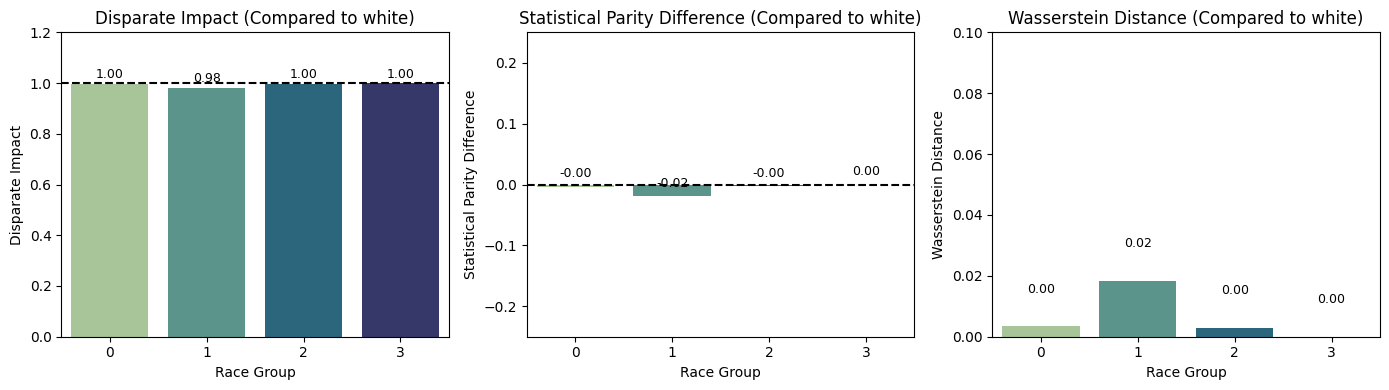
\includegraphics[width=0.95\textwidth]{raceexamplegood.png}
  \vspace{0.7em}
  \textbf{Figure:} Bias in race feature after mitigation
\end{center}

If instead we implement the Disparate Impact remover in a "textbook", canonical way, the results appear to be much worse. The method does not artificially remove the bias by using both the individual and global disparate impact remover, but it adds the custom weights to the training part, computing weights for a single protected attribute to rebalance joint label/protected group distribution, as well as individual weights. This aims to give weights to the protected features so that the model does not overly rely on those to make predictions, both in an individual and group way to avoid learning from bias as much as possible. 

This is a very standard technique, but it is evident that the results are not as satisfactory as we saw with the previous method. For the Family Income and Tier features, actually, the results all respect the 80\% rule, which indicates that the bias has been removed. while for the Race feature the situation is a lot more challenging. A reason behind this could be that the representation bias is harsher in this case, meaning that the number of white people in the database is much greater than all the other instances combined. This makes it much harder to remove the bias. 

\begin{center}
\captionof{table}{Logistic Regression classic DIR}
\begin{tabular}{llrr}
\toprule
\textbf{Attribute} & \textbf{Group} & \textbf{Disparate Impact} & \textbf{Statistical Parity Difference} \\
\midrule
\textbf{Race}
& 0 & 0.8267 & -0.1487 \\
& 1 & 0.4401 & -0.4805 \\
& 2 & 0.6738 & -0.2799 \\
& 3 & 0.7701 & -0.1972 \\
\midrule
\textbf{Family income}
& 1.0 & 0.7661 & -0.1919 \\
& 2.0 & 0.8992 & -0.0827 \\
& 3.0 & 0.9647 & -0.0289 \\
& 4.0 & 1.0262 & 0.0215 \\
\midrule
\textbf{Tier}
& 1 & 0.8668 & -0.1194 \\
& 2 & 0.8516 & -0.1330 \\
& 3 & 0.8716 & -0.1150 \\
& 4 & 0.9187 & -0.0729 \\
& 5 & 0.9088 & -0.0817 \\
\bottomrule
\end{tabular}
\end{center}

The reason why this method works great, is because Logistic Regression is a linear model that predicts the log-odds of an outcome as a weighted sum of the input features. Because of its linearity and simplicity, Logistic Regression is highly sensitive to the scale and distribution of input features. This makes it an excellent candidate for DIR. 

For the other two models, instead, adopting the textbook or classical approach does not matter much, as they do not reach the expected threshold.

In the Random Forest case, even if all features perform worse than seen in logistic regression, only the Race does not reach the acceptable value of 80\%, while the same cannot be said of XGBoost, which instead underperforms in all categories. 

\begin{center}
\captionof{table}{Random Forest}
\begin{tabular}{llrrr}
\toprule
Attribute & Group & Disparate Impact & Stat. Parity Diff.
\midrule
\textbf{Race}
& 0 & 0.8402 & -0.1420 \\
& 1 & 0.4947 & -0.4490 \\
& 2 & 0.6986 & -0.2678 \\
& 3 & 0.8190 & -0.1609 \\
\midrule
\textbf{Family Income}
& 1.0 & 0.7919 & -0.1790 \\
& 2.0 & 0.8886 & -0.0959 \\
& 3.0 & 0.9613 & -0.0333 \\
& 4.0 & 1.0148 & 0.0128 \\
\midrule
\textbf{Tier}
& 1 & 0.8073 & -0.1739 \\
& 2 & 0.8714 & -0.1161 \\
& 3 & 0.9167 & -0.0752 \\
& 4 & 0.9448 & -0.0498 \\
& 5 & 0.9534 & -0.0420 \\
\bottomrule
\end{tabular}
\label{tab:fairness_alternative_config}
\end{center}

\begin{center}
\captionof{table}{XGBoost}
\begin{tabular}{llrr}
\toprule
\textbf{Attribute} & \textbf{Group} & \textbf{Disparate Impact} & \textbf{Statistical Parity Difference} \\
\midrule
\textbf{Race}
& 0 & 0.7520 & -0.1991 \\
& 1 & 0.2267 & -0.6207 \\
& 2 & 0.5625 & -0.3512 \\
& 3 & 0.7123 & -0.2309 \\
\midrule
\textbf{Family Income}
& 1.0 & 0.6526 & -0.2650 \\
& 2.0 & 0.8338 & -0.1268 \\
& 3.0 & 0.9394 & -0.0462 \\
& 4.0 & 1.0273 & 0.0208 \\
\midrule
\textbf{Tier}
& 1 & 0.4248 & -0.4908 \\
& 2 & 0.7342 & -0.2268 \\
& 3 & 0.8361 & -0.1399 \\
& 4 & 0.9129 & -0.0744 \\
& 5 & 0.8989 & -0.0862 \\
\bottomrule
\end{tabular}
\end{center}


Contrarily to LR, both Random Forest and XGBoost are nonlinear ensemble models that can capture complex interactions and subtle patterns in the data. They tend to reconstruct the underlying patterns therefore bypassing the fairness constraints and still learning the bias. This makes it much harder to remove bias in them by only acting on the data, without touching the models themselves. Furthermore, we see that the protected feature that most poses a challenge to all models is race, which is also the one with the most unbalanced distribution. This information adds important context to the observed disparities, as it suggests that the models may be disproportionately influenced by the overrepresentation or underrepresentation of certain racial groups. As a result, even after bias mitigation techniques are applied, residual inequities may persist due to insufficient diversity in the underlying data



\subsubsection{In-processing}
The technique we've decided to use in order to remove bias from the best models previously found is the \textbf{Exponentiated Gradient}. It's a fairness-aware reduction technique and it solves a constrained optimization problem: it tries to maximize accuracy while satisfy fairness constrain. It does this by training an ensemble of classifiers. The fairness constraint that will be used in this mitigation technique is the \textbf{Demographic Parity}.\\ \\
For each model, the constraint has first been set over one biased feature at time, then all of them together.
\paragraph{Logistic Regression}\mbox{}\\


\section{Results}
In this study, we have demonstrated that algorithmic bias in educational datasets can be effectively mitigated, particularly through the use of in-processing techniques.
Our findings reinforce the growing consensus in the fairness research community: that modifying the learning algorithm itself, rather than simply adjusting the data, yields more robust and scalable fairness outcomes. Inprocessing techniques are effectively controlling the behaviour of the model itself, having a direct access to the model's optimization loo, which allows for optimization of the trade-off between fairness and accuracy. The inprocessing techniques also can adapt dynamically to the data distribution and model's performance, while preprocessing techniques only rely on the static modification of the data. We have showed that this data manipulation can work on less refined and more "gullible" models, but not on the more advanced ones, which is a great downside. Furthermore, preprocessing may introduce irreversible distortions or oversimplifications in the data that degrade the model’s ability to learn generalizable patterns.

Lastly, we find worth mentioning that according to previous research (\href{https://www.researchgate.net/publication/387044808_Fair_and_Transparent_Student_Admission_Prediction_Using_Machine_Learning_Models#read}{Fair and Transparent Student Admission Prediction Using Machine Learning Models}) Logistic Regression proved to be the fairest model to use in this context. This model is, as previously mentioned, extremely simple and transparent, which are huge upsides. On the other hand, though, it is necessary to underline that our dataset has a relatively small number of features. This is giving LR an advantage compared to the other models, but it is of high importance to investigate its behaviour in a more complex case. Still, it seems that our study further enhances the hypothesis advanced by G. Raftopoulos et al. which puts this model at the top of the fairness hierarchy for educational admission prediction tasks. However, it is important to emphasize that such a conclusion may not generalize across all educational contexts or datasets. 


\section{Conclusions and Future Work}

The previously commented results are especially important in the context of education, where algorithmic decisions can influence learners' trajectories, opportunities, and trust in automated systems. Making sure that these systems are as fair as possible is not only a technical challenge, but a social imperative given the tendency of automated systems to absorb historical biases. 

Looking ahead, we recommend that the following ideas are explored in future works: 
\begin{itemize}
    \item We recommend that also postprocessing techniques are tested on this specific dataset, to see if the results can be further improved.
    \item The models implemented should be tested on a variety of datasets, both in the United States context and abroad, to check how the bias presents itself. This is a question of transfer learning, and it is a current topic of research in machine learning and fairness fields.
    \item The models and code should be tested in a real-world scenario instead of on artificial data such as in this case. Even if this dataset is as realistic as it can be, the real-world implications should be studied as well.
    \item Investigation on Logistic Regression should be conducted, both from a theoretical and empirical point of view, to understand how the use of this specific machine learning model impacts fairness, and wether it is too oversimplistic to be used in real world scenarios. 
\end{itemize}

Ultimately, we strive to achieve a future where educational ML systems do not only avoid harm, but ensure equity and inclusiveness. Our study is a small step in this direction and we hope it can be a foundation for future research in this field. 




\bibliographystyle{plainurl}
\bibliography{sample}

\end{document}